\documentclass[12pt, a4paper]{report}

% --- Packages ---
\usepackage[utf8]{inputenc}
\usepackage[T1]{fontenc}
\usepackage{microtype}
\usepackage{amsmath, amssymb}
\usepackage{graphicx}
\graphicspath{{../figures/}{./figures/}}
\usepackage{geometry}
\usepackage{setspace}
\usepackage{hyperref}
\usepackage{booktabs}
\usepackage{caption}
\usepackage{subcaption}
\usepackage{float}
\usepackage{enumitem}
\usepackage[backend=biber, style=ieee]{biblatex}
\addbibresource{references.bib}

% Allow line breaks in URLs and DOIs to fix overfull \hbox
\setcounter{biburllcpenalty}{7000}
\setcounter{biburlucpenalty}{8000}

% --- Page Setup ---
\geometry{
    top=1in,
    bottom=1in,
    left=1.5in, % Margin for binding
    right=1in
}
\setstretch{1.5} % 1.5 line spacing for thesis readability

% --- Title Page Info ---
\title{
    \textbf{\Large Tactile-Feedback Teleoperation: Grip Force and Grasping Performance Across Haptic Actuator Types for Fragile and Deformable Objects}\\
    \vspace{1cm}
    \large Bachelor's Thesis
    \vspace{1cm}
}

\author{
    \textbf{Adriel I. Santoso}\\
    Department of Mechanical and Aerospace Engineering\\
    Tohoku University
}

\date{
    \vspace{2cm}
    \today
}

\begin{document}

\maketitle

\pagenumbering{roman}

\begin{abstract}
    \addcontentsline{toc}{chapter}{Abstract}
    Teleoperation of robotic systems, such as pick-and-place tasks, often suffers from a lack of haptic feedback, forcing operators to rely entirely on visual cues. This reliance can lead to the application of excessive force, damaging delicate objects, or insufficient force, leading to slippage. This thesis investigates a teleoperation framework that integrates a Robotiq 2F-85 Adaptive Gripper equipped with vision-based stress-deformation tactile sensors (9DTact) into the fingertip contact surfaces. The tactile data generated during grasping is translated in real time into haptic feedback delivered to the operator through a custom five-channel wearable actuator array driven by an ESP32-C6 microcontroller. Two mechanically distinct actuator types are evaluated under an identical sensing and control pipeline: linear resonant actuators (LRAs), driven by a bipolar resonant carrier whose envelope encodes the intensity signal, and TacTiles bistable pin actuators, driven by short latching H-bridge pulses. Through quantitative grip-force and grasp-quality measurements and qualitative participant surveys, this study compares LRA and TacTiles feedback against a visual-only baseline during the manipulation of fragile and deformable objects. Results aim to determine whether either actuator type meaningfully improves grip-force regulation and grasp outcomes relative to visual feedback alone, and whether the two actuation mechanisms differ in their suitability for continuous, proportional tactile rendering.
\end{abstract}

\pagebreak
\tableofcontents
\listoffigures
\listoftables
\pagebreak

\pagenumbering{arabic}

% ==========================================
% CHAPTER 1: INTRODUCTION
% ==========================================
\chapter{Introduction}

\section{Background and Motivation}
Teleoperated robotic systems have become integral to settings where direct human presence is impractical or unsafe, including nuclear decommissioning, minimally invasive surgery, and the handling of hazardous materials. In industrial manufacturing, teleoperation enables human-robot collaboration, in which the operator guides the robot through a command channel while the robot streams sensory information back through a feedback channel \cite{zheng2024}. Medical applications extend this paradigm to microsurgery and remote procedures, where a clinician manipulates a master console and a robot reproduces those motions with scaled precision. These domains share a common requirement: the operator must perceive the remote environment accurately to execute tasks efficiently and safely \cite{huang2019}.

A persistent limitation of conventional teleoperation systems is that the operator receives little or no tactile information from the remote end-effector. Visual feedback conveys spatial position and gross motion, but it does not communicate contact forces, surface compliance, or slip, which are cues humans rely on instinctively during everyday object manipulation. The absence of this tactile channel becomes critical when the task involves fragile or compliant objects, such as assembling delicate electronic components or grasping soft tissue during robotic surgery \cite{zheng2024}. Haptic feedback addresses this gap by rendering contact forces at the master side, allowing the operator to feel the interaction remotely. Reducing this sensory deficit may lower cognitive load, improve precision, and reduce the likelihood of unintended damage \cite{zheng2024}. Yet the design of effective haptic interfaces for teleoperation remains an open engineering challenge, and the choice of actuator hardware used to render that feedback is itself an underexplored design variable.

\section{The Role of Touch in Human Grasping}
During object manipulation, humans regulate grip force through a control architecture that depends critically on tactile afferent signals from the fingertips. Cutaneous mechanoreceptors in the finger pads, specifically rapidly adapting FA-I afferents (Meissner corpuscles) and slowly adapting SA-I afferents (Merkel cells), encode contact events, surface geometry, and frictional conditions with sufficient speed and resolution to inform motor output within roughly 100 milliseconds of contact \cite{johansson2009}. Rather than relying solely on reactive feedback, the central nervous system uses these tactile signals to support feedforward control: internal models of object properties are updated from prior sensory experience, enabling the motor system to predict the grip force required before lift-off and to preemptively adjust force ratios as load conditions change. This discrete-event, sensory-driven scheme means tactile information is not merely a corrective overlay but an integral part of the planning and execution of each manipulation phase.

When the same task is performed through a teleoperated robot, the operator's fingertips receive no contact information from the remote end-effector. The feedforward loop is severed: without the skin afferents that normally signal incipient slip, surface compliance, and contact timing, the operator cannot build or update the internal models that make delicate grasp control possible. This is not simply a matter of reduced fidelity or immersion. The human sensorimotor system is structurally dependent on tactile feedback for predictive grip-force regulation, and its absence eliminates a core mechanism through which dexterous manipulation is achieved \cite{johansson2009}.

\section{Existing Haptic Feedback Approaches \& Their Limitations}
Haptic feedback for teleoperation can be delivered through several distinct modalities, each with characteristic trade-offs in fidelity, form factor, and practical deployability. Kinesthetic (force-feedback) interfaces reproduce contact forces at the joint level, offering high mechanical transparency, but require grounded or exoskeletal structures that are bulky, expensive, and difficult to wear outside a laboratory setting \cite{pacchierotti2017}. Electrotactile displays stimulate cutaneous afferents directly via surface electrodes, enabling finely patterned tactile sensations with minimal mechanical hardware; however, they suffer from sensitivity to skin hydration, discomfort at sustained stimulation levels, and limited perceptual bandwidth. Thermal haptic feedback, while useful for conveying material properties such as thermal conductivity, is intrinsically slow to change and cannot support the rapid transients needed for grip-force regulation.

Within the broader category of mechanical cutaneous actuation, two device classes are of particular interest for compact, multi-channel wearable arrays. Linear resonant actuators (LRAs) drive a spring-mounted moving mass with a voice coil to produce vibration along a single axis; they are compact, low-mass, drivable from simple electronics, and, because they operate at a fixed mechanical resonance, can vary vibration intensity without the amplitude–frequency coupling that constrains the eccentric-rotating-mass (ERM) motors used in most earlier vibrotactile work \cite{pacchierotti2017}. A mechanically distinct alternative is the bistable, latching pin actuator, exemplified by the TacTiles design of Vechev et al., which uses asymmetric electromagnetic latching to hold a pin in one of two stable states without continuous power draw \cite{vechev2019}. Because a bistable actuator consumes energy only during a state transition rather than for the duration of a stimulus, this class offers a fundamentally different power and temporal-response profile from a continuously-driven resonant actuator, while still being realizable as a compact, multi-channel array suitable for fingertip-scale wearables \cite{vechev2019}. These contrasting profiles, smooth proportional drive at a fixed resonant frequency for the LRA, and crisp, discrete contact events with low average power for the bistable pin actuator, motivate a direct comparison of the two when rendering continuous tactile sensor data in a teleoperation loop \cite{choi2013}.

Despite the prevalence of vibrotactile feedback, most teleoperation systems that use it rely on a binary actuation paradigm: each tactor is either on or off, typically triggered by a force threshold at the remote end-effector. This conveys only a single bit of information per contact point, namely whether contact has occurred, and discards the continuous force, direction, and texture signals the human tactile system uses to regulate grip. Choi and Kuchenbecker \cite{choi2013} note that while vibrotactile perception supports parametric encoding of intensity, frequency, and temporal pattern, most systems fail to exploit these dimensions. A critical gap therefore persists: available haptic interfaces for teleoperated grasping rarely render a continuous, proportional mapping from measured contact deformation to actuator drive signal, and prior comparisons between actuator types have not been conducted under a matched sensing and control pipeline that isolates the actuator hardware as the sole experimental variable \cite{pacchierotti2017}.

\section{Tactile Sensing on the Robot Side}
The quality of any haptic feedback interface is inherently bounded by the information content of the sensor signal from which it is derived. A common approach in commercial grippers such as the Robotiq 2F-85 is to estimate contact force indirectly through motor-current sensing: the gripper's control logic sets a current limit that corresponds to a desired gripping force, and an object-detection event is triggered when the current exceeds that threshold \cite{robotiq_manual}. This method yields a single scalar proxy for the total grip force applied across both fingers. It provides no information about how contact force is distributed across the fingertip surface, the geometry of the contact patch, or the location of incipient slip, all of which are critical cues for dexterous manipulation. When this scalar estimate is used as the sole input to a haptic display, the operator receives only an aggregate force reading, which cannot support spatially resolved feedback at individual contact points.

Vision-based gel deformation sensors offer a fundamentally richer alternative. These sensors, such as the GelSight family and the more recent 9DTact design, use a camera to observe the deformation of an elastomeric surface under contact, recovering a dense, continuous depth map proportional to local indentation rather than a single aggregate force value \cite{lin2023}. Whereas motor-current sensing collapses the entire contact interaction into one number, a vision-based tactile sensor preserves the spatial structure of the grasp: it encodes where on the fingertip the object is pressing, how the pressure gradient shifts during manipulation, and how that pattern evolves as the gripper closes. This depth map can be reduced to a scalar summary statistic, such as its maximum or mean value, for use as a control signal in a real-time feedback loop, while still retaining the option of full spatial rendering for future multi-channel mappings.

\section{Problem Statement}
Existing work on vibrotactile feedback for teleoperated grasping has predominantly used eccentric-rotating-mass motors as the sole actuator type, with the choice of actuator hardware rarely treated as an independent experimental variable \cite{pacchierotti2017}. On the sensing side, teleoperation systems that incorporate contact feedback have often relied on single-point force sensors or motor-current proxies, which measure total grip force without resolving its spatial distribution across the fingertip \cite{zheng2024}. Meanwhile, vision-based tactile sensors such as 9DTact have been developed for autonomous robotic manipulation tasks such as slip detection and shape reconstruction \cite{lin2023}, but their continuous depth output has not been systematically compared as the input to two mechanically distinct classes of wearable haptic actuator under otherwise identical conditions.

No prior work has implemented a teleoperation pipeline in which a vision-based tactile sensor mounted on a Robotiq 2F-85 gripper drives both a continuously-driven resonant actuator array (LRA) and a bistable pin actuator array (TacTiles) from the same real-time depth signal, allowing the two actuator technologies to be compared directly while holding the sensing and control software constant. Furthermore, no user study has compared continuous, sensor-driven LRA feedback and bistable pin feedback against a common visual-only baseline in a teleoperated grasping task involving fragile and deformable objects. Controlled experimental comparison across these three conditions, visual-only, LRA, and TacTiles, is therefore absent from the literature.

\section{Thesis Objectives}
This research aims to address the above gap through the following core objectives:
\begin{enumerate}
    \item To integrate and calibrate a vision-based tactile sensor (9DTact) into a Robotiq 2F-85 gripper, enabling continuous, real-time deformation measurement at the fingertip contact surface.
    \item To develop low-latency firmware on an ESP32-C6 microcontroller that drives two mechanically distinct actuator arrays, namely five LRA channels driven by a bipolar resonant carrier and five TacTiles bistable pin actuator channels driven by latching H-bridge pulses, from a common sensor-derived intensity signal.
    \item To evaluate operator performance and subjective experience in a teleoperated grasping task involving fragile and deformable objects under three feedback conditions, namely visual-only feedback, LRA vibrotactile feedback, and TacTiles bistable feedback, through a within-subjects user study.
\end{enumerate}

\section{Thesis Structure}
Chapter 1 introduces the motivation for haptic feedback in robotic teleoperation, presents the research problem, and states the thesis objectives. Chapter 2 reviews the relevant literature on tactile sensing for robotic grasping and the two haptic actuator technologies under study, identifying the gap in direct, sensor-matched comparisons between continuously-driven and bistable actuator types for teleoperation. Chapter 3 describes the system architecture, including the integration of the 9DTact tactile sensor onto a Robotiq 2F-85 gripper communicating over Modbus RTU and the design of an ESP32-C6-based driver supporting both LRA and TacTiles actuator channels from a shared sensing pipeline. Chapter 4 outlines the experimental methodology, detailing the teleoperated grasping task design, the three feedback conditions (visual-only, LRA, and TacTiles), and the survey instruments for subjective workload and experience measures. Chapter 5 presents the results, including system latency benchmarks from the sensor-to-actuator pipeline for each actuator type and statistical analysis of both objective grasp-quality metrics and Likert-scale survey data. Chapter 6 interprets these findings in the context of the literature, discusses the practical implications for selecting haptic actuator hardware in teleoperation interface design, and acknowledges the limitations of the study. Chapter 7 concludes the thesis by summarizing the contributions and proposing directions for future work, including possible connections to energy-based modeling frameworks for analyzing the teleoperation loop.

% ==========================================
% CHAPTER 2: LITERATURE REVIEW
% ==========================================
\chapter{Literature Review}

\section{Robotic Grasping and Force Feedback}
Force sensing has been established as a prerequisite for stable robotic grasping across the entire spectrum of end-effector complexity, from industrial parallel-jaw grippers to multi-fingered dexterous hands. In industrial pick-and-place applications, contact force information enabled binary object detection and prevented damage by limiting the maximum force applied to rigid workpieces \cite{dahiya2010}. As end-effectors became more dexterous, the sensing requirements shifted from simple force thresholds to spatially-resolved tactile information. Multi-fingered hands and compliant manipulators required knowledge of contact location, force direction, and pressure distribution across each fingertip to regulate the balance between normal and shear forces during in-hand manipulation \cite{dahiya2010}. Tactile sensor arrays placed close to the contact interface provided this distributed measurement, enabling grasp stability assessment and slip detection at rates that closed-loop vision could not match. Without this spatial force information, dexterous control strategies such as compliant grasping and adaptive force regulation were reduced to open-loop or vision-guided heuristics.

The Robotiq 2F-85 adaptive gripper exemplifies both the capabilities and the limitations of force sensing in an industrial-grade end-effector. Its fingers are underactuated: a single motor drives both fingers through a four-bar linkage, and the mechanical compliance of the two-phalanx finger design allows the gripper to self-adapt between pinch and encompassing grasp modes depending on the contact point on the fingertip \cite{robotiq_manual}. To estimate grip force, the gripper relies on motor-current monitoring: the force setpoint is translated into a current limit, and the controller registers an object-detection event when the current exceeds that threshold during finger closure \cite{robotiq_manual}. This returns a single aggregate scalar correlated with the total resistance encountered by the actuator. It cannot resolve how that force is distributed across the two phalanxes of each finger, nor distinguish a stable distributed grasp from a point contact on the fingertip edge. For compliant or fragile objects, where maintaining an even pressure distribution across the contact surface is critical to avoid local deformation or damage, this aggregate measurement is fundamentally insufficient. The absence of spatially-resolved tactile information means the controller cannot distinguish a safe conforming grasp from one that applies excessive local force, limiting the gripper's suitability for dexterous manipulation of soft, brittle, or irregularly-shaped objects \cite{dahiya2010}. This thesis addresses that limitation directly by augmenting the 2F-85 with a vision-based tactile sensor at the fingertip, described in the following section.

\section{Vision-Based Tactile Sensing}
Tactile sensor technologies for robotic fingertips differ substantially in transduction principle, spatial resolution, and the practical difficulty of integrating them into a compact end-effector. Piezoresistive sensors, based on materials whose electrical resistance decreases under mechanical compression, can be fabricated as dense MEMS arrays with spatial resolution approaching 1~mm, but they suffer from hysteresis, temperature drift, and the inherent fragility of silicon substrates under the forces encountered during routine grasping \cite{dahiya2010}. Capacitive tactile sensors transduce pressure through changes in electrode spacing or dielectric properties, achieving fine taxel pitches, and their compatibility with flexible printed-circuit substrates allows conformable integration onto curved fingertip surfaces, though the signal chain requires careful shielding against parasitic capacitance and noise \cite{dahiya2010}. Vision-based gel deformation sensors, such as the GelSight family, use a camera to observe the deformation of an elastomeric surface under contact, recovering 3D contact geometry at micrometre-level resolution through photometric stereo or marker tracking; this approach delivers the highest spatial resolution of any tactile modality, but the need for an embedded camera, directional illumination, and computational processing for 3D reconstruction imposes significant constraints on sensor thickness, cabling, and manufacturing reproducibility \cite{donggelsight2021}.

The 9DTact sensor used in this work belongs to this vision-based family, but is designed specifically for compact, repeatable fabrication and fingertip-scale integration onto standard grippers \cite{lin2023}. Rather than producing a sparse taxel grid, it recovers a dense depth map of the contact surface at standard video frame rates, from which scalar summary statistics, such as the maximum indentation depth across the contact patch, can be extracted with low latency for use as a real-time control signal. The trend toward compact vision-based sensors such as 9DTact demonstrates that this sensing approach can be fabricated with repeatable assembly processes, fitted to the fingertip form factor of standard grippers, and operated at update rates sufficient for closed-loop teleoperation, suggesting that constraints on fragile substrates and complex packaging need not preclude deployment in practical end-effectors \cite{lin2023}.

\section{Tactile Sensing for Slip Detection and Manipulation}
Tactile sensor arrays have been applied extensively to three interrelated perception tasks in robotic manipulation: slip detection, grasp stability assessment, and object shape reconstruction \cite{dahiya2010}. A substantial body of work used the high-resolution spatial contact maps produced by vision-based gel sensors to detect incipient slip before gross motion occurred, for example by monitoring the shear-induced deformation of a gel surface through marker tracking or photometric stereo, enabling a robot controller to increase grip force preemptively \cite{donggelsight2021}. GelSight-type sensors proved particularly influential here: their ability to recover sub-millimetre 3D contact geometry from a single tactile image made them well suited to estimating object pose during manipulation, assessing whether a grasp was centred and stable, and detecting the onset of rotational or translational slip from the deformation of the contact patch \cite{donggelsight2021}. In parallel, compact designs such as GelSlim 3.0 integrated shape reconstruction, force distribution estimation, and incipient slip detection into a single fingertip-sized module, demonstrating that a robot could use these combined tactile signals to maintain stable grasps on objects of varying geometry and compliance without dropping or damaging them \cite{taylor2021}. The 9DTact sensor further extended this paradigm by combining 3D shape reconstruction with 6D force estimation from a learned deformation representation, enabling a robot to infer both the geometry of the contacted surface and the full force vector applied to it \cite{lin2023}.

Across all of these efforts, the consumer of the tactile data was an autonomous robot controller: a policy, a feedback loop, or a state estimator that acted on the sensor output directly by adjusting motor commands. This assumption was sensible for autonomous manipulation, but it meant sensor outputs were optimised for machine-readable properties such as regression accuracy for force vectors or classification accuracy for slip events, not for human perceptual interpretability. The depth maps and deformation fields these sensors produced were not systematically evaluated as the input to a human haptic display in a teleoperation loop, where the operator must interpret tactile cues through a wearable actuator array rather than through an automated controller, and where the choice of actuator hardware itself shapes what can be perceived. This gap motivates a review of the haptic feedback methods and actuator technologies developed for teleoperation interfaces, addressed in the following sections.

\section{Haptic Feedback in Teleoperation}
Haptic feedback in teleoperation was first realised through grounded kinesthetic interfaces, which rendered contact forces at the master console by mechanically coupling the operator's hand to a rigid base. Commercial devices such as the Phantom series and the Omega 3 provided three or more degrees of freedom of force feedback with sub-millimetre positioning accuracy, enabling tasks ranging from needle insertion to remote palpation \cite{pacchierotti2017}. These grounded masters offered high mechanical transparency because the reaction forces from actuation were absorbed by the ground rather than by the operator's body, preserving the illusion of direct contact with the remote environment \cite{pacchierotti2017}. However, this fidelity came at the cost of substantial size, weight, and expense: typical grounded haptic devices weighed several kilograms and required dedicated mounting surfaces, confining them to laboratory benchtops and clinical research settings \cite{pacchierotti2017}. Their form factor also limited multi-contact interaction; grasping a two-fingered object would have required multiple grounded devices, which was impractical outside a controlled setup \cite{pacchierotti2017}. These constraints motivated the exploration of lighter, ungrounded alternatives that could be worn directly on the operator's hand.

Cutaneous haptic interfaces emerged as a compelling alternative precisely because they eliminated the need for a grounded reaction mass. Cutaneous devices applied forces directly to the skin, rendering contact pressure, shear, and stretch without generating reaction torques that had to be supported by an external structure \cite{pacchierotti2015}. By keeping the feedback ungrounded, these devices contributed to loop stability even in the presence of communication delays or hard contacts, making them especially attractive for medical and safety-critical applications \cite{pacchierotti2017}. Within this cutaneous category, two mechanically distinct actuation strategies are evaluated in this thesis and are reviewed in turn below.

\section{Linear Resonant Actuators}
A linear resonant actuator (LRA) drives a spring-mounted moving mass with a voice coil, producing vibration along a single axis. Unlike an eccentric-rotating-mass motor, whose amplitude and frequency are mechanically coupled through a single DC drive level, an LRA is driven by an alternating signal at or near the fixed resonant frequency of its mass--spring system, so perceived amplitude can be modulated through drive level while the vibration frequency stays essentially constant \cite{pacchierotti2017}. This decoupling is attractive for rendering a pure intensity signal such as contact depth, because intensity can be varied without the frequency drift that accompanies duty-cycle modulation of an ERM. The trade-off is a narrow usable bandwidth: an LRA is efficient only in a small band around its resonance, and reaching or leaving full amplitude requires several drive cycles of mechanical ring-up and ring-down, which bounds how quickly the rendered intensity can change. Because LRA resonant frequencies commonly fall in the 150--250~Hz range, they sit near the peak sensitivity of the Pacinian channel, where detection thresholds on glabrous skin are lowest, following the U-shaped threshold-versus-frequency curve that reaches its minimum around 250--300~Hz \cite{verrillo1985}; this places the LRA's operating point in a favourable region for fingertip vibrotactile rendering. These properties, low mass, simple drive electronics, and intensity modulation at a stable frequency, made the LRA the continuously-driven actuator selected for this study, and several recent teleoperation gloves have likewise adopted LRA arrays for sensor-driven feedback \cite{luo2024}.

\section{TacTiles Bistable Pin Actuators}
Bistable, latching pin actuators represent a mechanically distinct approach to cutaneous stimulation. Vechev et al.\ introduced TacTiles, light (1.8~g), low-power (130~mW), and small form-factor (1~cm$^3$) electromagnetic actuators that use a custom multi-layer PCB coil and asymmetric magnetic latching to hold a pin in one of two stable mechanical states without continuous power draw \cite{vechev2019}. Their design supports two distinct drive modes: a contact mode, in which the pin is driven and held against the skin to render sustained, static contact, and a pulse mode, in which the pin is rapidly engaged and retracted to render discrete tactile events; both modes were shown to be reliably localisable and discriminable by users in a virtual-reality rendering task \cite{vechev2019}. Because the actuator consumes energy only during a state transition rather than for the duration of a stimulus, this class offers a fundamentally different power and temporal-response profile from a continuously-driven resonant actuator, while still being realizable as a compact, multi-channel array suitable for fingertip-scale wearables \cite{vechev2019}. A continuous-feeling vibration can be approximated on this hardware by issuing repeated engage/disengage or pulse cycles at a controlled rate, at the cost of a hardware-imposed upper bound on sustainable switching frequency before thermal or mechanical limits are reached.

Pin-based actuators more broadly have also been explored for spatial shape and texture rendering: Wu et al.\ combined a pin array with conventional vibration motors in a single wearable device, finding that the pin array excelled at conveying shape and fine-texture information that vibrotactile actuation alone could not reproduce, while the combination of both mechanisms gave the most realistic rendering of coarse textures and dynamic patterns \cite{vipins2025}. This complementary relationship between displacement-based and vibration-based cutaneous stimulation motivates a direct, matched comparison between an LRA array and a TacTiles bistable pin array when both are driven by the same underlying tactile sensor signal, which is the core empirical contribution of this thesis.

\section{Comparative Gap: Continuous Versus Bistable Actuation for Teleoperated Grasping}
Several research groups have explored sensor-driven haptic feedback for teleoperated grasping, with systems varying in sensor type, actuator configuration, and mapping policy, but in nearly every case the actuator hardware itself was fixed rather than treated as an independent variable. Luo et al.\ \cite{luo2024} presented textile-based smart gloves integrating piezoresistive force sensors and linear resonant actuator arrays, in which a pressure-sensing matrix on a Robotiq 2F-140 gripper was mapped to vibrotactile units on the operator's hand using a binary, threshold-triggered scheme; a ten-participant study showed that even this coarse mapping enabled stable grasping without visual feedback, but the comparison did not extend to a second actuator technology. García-Robledo et al.\ \cite{garciarobledo2011} proposed a vibrotactile glove for depth perception in teleoperation, using five ERM motors whose amplitude scaled with measured distance rather than contact force; a within-subjects study against a visual-only baseline found faster task completion with haptic cues present, though the improvement was not statistically significant across all metrics. Abdi et al.\ \cite{abdi2020} combined a wrist-mounted force-torque sensor with vibrotactile armbands driven proportionally by force magnitude, finding significant reductions in collision count and peak contact force relative to a no-feedback baseline.

Tsetserukou et al.\ \cite{tsetserukou2010} used a Kinotex fiber-optic tactile array discretised into three intensity levels, delivered through DC-motor-driven actuators, but the mapping remained strictly stepped rather than continuous. Pacchierotti et al.\ \cite{pacchierotti2015b} moved away from vibrotactile actuation entirely, developing a cutaneous fingertip device that rendered deformation proportional to aggregate force-torque readings in a teleoperated peg-in-hole task, finding that cutaneous feedback stabilised the teleoperation loop under communication delays. None of these studies, however, evaluated more than one mechanically distinct actuator type within the same experimental pipeline, and none used a vision-based tactile sensor capable of producing a continuous, real-time intensity signal suitable for driving both a continuously-modulated actuator and a discretely-switched bistable actuator under matched conditions.

This represents a clearly defined gap: whether a continuously-driven actuator such as an LRA or a discretely-switched bistable actuator such as a TacTiles pin better supports grip-force regulation and grasp quality when both are driven by the same vision-based tactile sensor signal during teleoperated manipulation of fragile and deformable objects remains an open question. The system architecture developed to investigate this question is described in Chapter~\ref{ch:architecture}.

% ==========================================
% CHAPTER 3: SYSTEM ARCHITECTURE
% ==========================================
\chapter{System Architecture}
\label{ch:architecture}
\section{Overall Framework Design}
\label{sec:framework}
The system implements a closed sensorimotor teleoperation loop bridging a robotic end-effector and a human operator's hand, built around three nodes: a host PC, the Robotiq 2F-85 gripper, and an ESP32-C6 microcontroller worn by the operator. The host PC runs the main control process (\texttt{experiment.py}) inside the project's \texttt{hapticf} Python environment (Python 3.10, CUDA 13.0), which consolidates the full CUDA, SciPy, Open3D, MediaPipe, and gripper-communication dependency stack required by the 9DTact reconstruction library into a single environment.

At each control tick, the host performs three reads and one computation before issuing two writes. It reads the Robotiq 2F-85's position and motor-current registers (\texttt{gPO}, \texttt{gCU}) over Modbus RTU via a USB-to-RS485 adapter; it reads a hand-tracking webcam frame and runs MediaPipe hand-landmark detection to determine the operator's intended grip aperture; and it reads the 9DTact tactile sensor mounted on the gripper's fingertip, obtaining a calibrated height map of the current contact deformation. From the height map, a single scalar haptic intensity value is computed as the maximum indentation depth across the contact patch, normalised against a configurable saturation depth and clamped to the interval $[0,1]$. This intensity value is streamed over USB serial to the ESP32-C6 at a fixed rate, while the hand-tracking-derived target aperture is simultaneously written back to the gripper's position register: the operator's hand motion drives the gripper, and the gripper's resulting tactile contact is rendered back to the operator's hand.

The ESP32-C6 is agnostic to which physical actuator array is attached; it decodes the incoming intensity stream and renders it through whichever array is currently wired to its GPIO pins, either the LRA array or the TacTiles bistable pin array, using a common text streaming protocol described in Section~\ref{sec:driver}. This design deliberately isolates the actuator hardware as the only difference between the two haptic feedback conditions: the sensing pipeline, the intensity computation, the communication protocol, and the gripper control logic are identical across both, and only the firmware rendering mode and the physical actuator array attached to the ESP32-C6 change between conditions. Figure~\ref{fig:arch} summarises this architecture.

\begin{figure}[h]
    \centering
    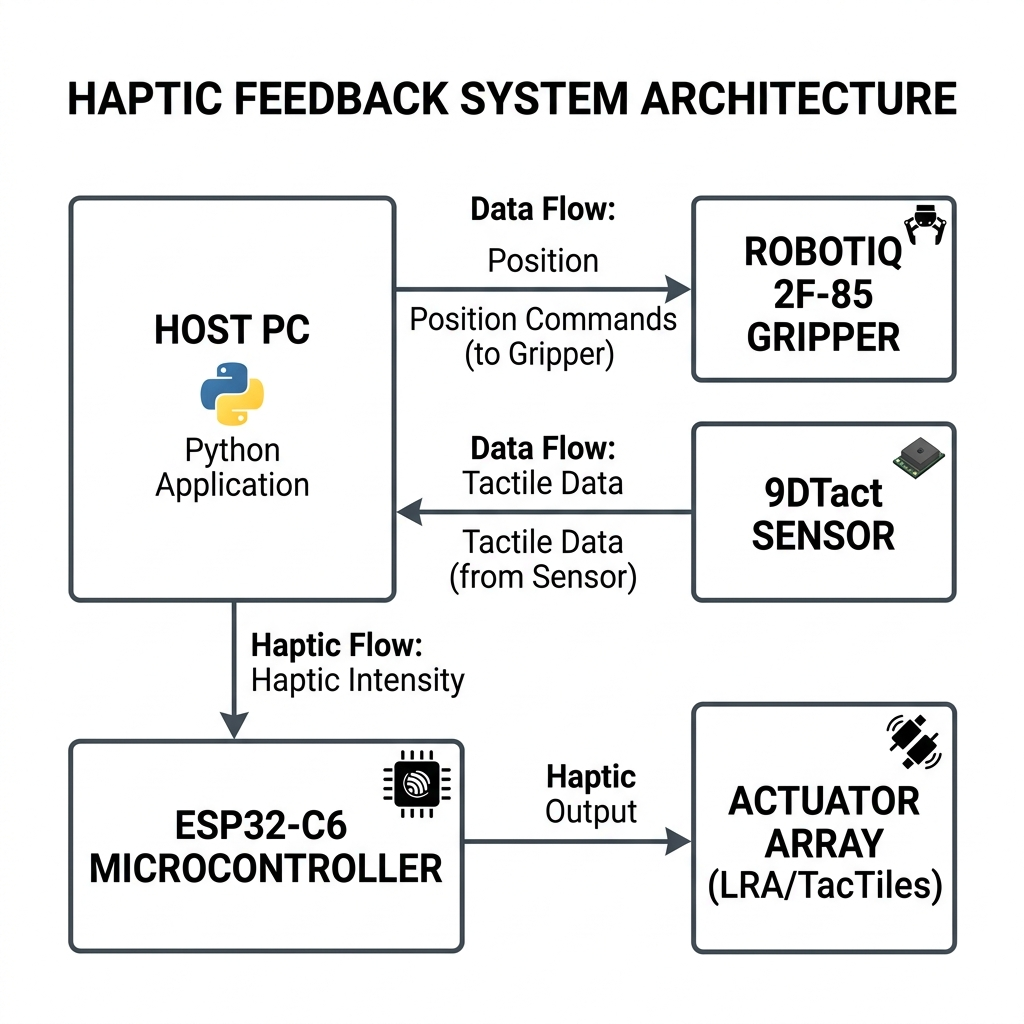
\includegraphics[width=0.8\textwidth]{system_architecture.png}
    \caption{System block diagram: the host PC reads gripper state, hand-tracking video, and 9DTact tactile data, computes a target gripper position and a scalar haptic intensity, and writes the former to the gripper over Modbus RTU and the latter to the ESP32-C6 over USB serial. The ESP32-C6 renders the intensity through either the LRA or TacTiles actuator array.}
    \label{fig:arch}
\end{figure}

\section{Robotiq 2F-85 and Tactile Integration}
The primary manipulation hardware is the Robotiq 2F-85 adaptive gripper, communicating with the host PC over Modbus RTU at 115200 baud via a USB-to-RS485 adapter, using the \texttt{pyRobotiqGripper} Python library. Before any position command can be issued, the gripper must complete an activation sequence: the host writes the activation request bit (\texttt{rACT}) and then polls the gripper status register (\texttt{gSTA}) until it reports a value of 3, indicating activation is complete. To avoid unnecessarily re-triggering the gripper's internal auto-calibration sweep, which occasionally caused activation to exceed its timeout window during testing, the control software first reads \texttt{gSTA} and issues a fresh activation (preceded by an explicit reset) only if the gripper is not already activated, rather than calling activate unconditionally on every program start.

Once activated, position, speed, and force setpoints are issued as a single Modbus write to a contiguous block of holding registers: an action-request word encoding go-to and activation bits, followed by a target position (0--225) and a combined speed/force byte pair. Gripper state is read back via the same interface into a parameter dictionary populated by \texttt{readAll()}, exposing the current position (\texttt{gPO}) and the instantaneous motor current (\texttt{gCU}). The latter is the only force-related signal the 2F-85 natively provides: the gripper has no force or torque sensor, and \texttt{gCU} is a coarse, single-channel proxy for the total resistance encountered by the underactuated drive motor across both fingers. This proxy cannot resolve how contact force is distributed across the fingertip surface, motivating the addition of a dedicated tactile sensor at the point of contact, described next.

\subsection{Sensor Integration and Calibration}
\label{subsec:sensorcalib}
A 9DTact vision-based tactile sensor is mechanically affixed to the fingertip contact surface of the gripper's left finger. Bringing a 9DTact sensor into a usable state requires two independent calibration stages, performed once per physical sensor unit and stored per-sensor (left and right sensors are calibrated and stored separately, since manufacturing variation in gel thickness and camera focus produces measurably different calibration curves between nominally identical units).

The first stage, camera calibration, corrects for lens distortion and establishes a physical pixel-to-millimetre scale. With nothing touching the sensor, a reference frame is captured; a printed dot-grid calibration board is then pressed flat against the gel surface and a sample frame captured. The two frames are differenced and thresholded to isolate the indentation produced by each grid dot, and the centroid of each resulting contour is taken as a detected grid point. Given the known physical spacing between grid points, the average pixel distance between adjacent detected points yields a pixel-per-millimetre scale factor, and a radial basis function interpolation between the detected (distorted) point positions and their expected (undistorted) regular-grid positions produces a per-pixel remapping table used to rectify all subsequent frames from that sensor.

The second stage, depth calibration, builds a lookup table mapping pixel brightness change to physical indentation depth. A ball of known radius is pressed onto the calibrated (rectified) sensor surface; the resulting circular contact patch is detected from the brightness difference relative to the no-contact reference frame, and the known spherical geometry of the indentation, together with the pixel-per-millimetre scale from camera calibration, is used to assign a physical depth value to each pixel within the contact circle. Aggregating depth as a function of brightness across the indentation produces the brightness-to-depth lookup table used during operation.

The two calibrated sensors used in this work exhibited materially different depth ranges: the left sensor's lookup table spanned approximately 1.33--2.60~mm, while the right sensor's spanned approximately 0.58--1.25~mm, despite nominally identical hardware. This was confirmed empirically before any data collection by verifying that, with nothing touching the sensor, the resulting height map was uniformly zero (mean, minimum, and maximum all equal to zero) and the underlying pixel-difference noise floor had a standard deviation below one grey level, ruling out a noisy or miscalibrated baseline as a confound in subsequent measurements. Once calibrated, each sensor returns a dense height map in millimetres at standard video frame rates, from which the maximum indentation depth across the contact patch is extracted as the scalar control signal driving the haptic feedback described in Section~\ref{sec:driver}.

\section{ESP32-C6 Haptic Driver}
\label{sec:driver}
On the operator side, the scalar haptic intensity value derived from the tactile sensor is rendered through whichever actuator array is physically attached to the ESP32-C6, either five LRA channels or five TacTiles pin actuator channels, with the choice of array determined by which experimental condition is being run rather than by any change to the host-side control software. The same intensity value is currently broadcast identically to all five channels; a spatially-resolved, per-region mapping across the sensor's depth map is left as future work (Chapter~\ref{ch:conclusion}).

Communication between the host and the ESP32-C6 uses a line-based text streaming protocol implemented in the board's MicroPython firmware. On each iteration the firmware performs a non-blocking check of standard input; when a complete newline-terminated line is available, it is read with \texttt{sys.stdin.readline()} and parsed as a single floating-point intensity value with \texttt{float()}, malformed lines being discarded. The host transmits one such line per update, formatted as \texttt{"\{intensity:.4f\}\textbackslash n"}, and the decoded value is applied to every channel in the active array. The firmware also maintains a watchdog: if no valid packet has been received within a 200~ms window, the rendered intensity is forced to zero, so a stalled or disconnected host process, or a crash on the host side, cannot leave an actuator energised indefinitely. Crucially, the watchdog drops the commanded intensity to zero while keeping the driver hardware awake, rather than fully powering the driver down; this avoids a failure mode in which a brief inter-packet gap puts the driver to sleep and subsequent packets arrive at an unresponsive chip. Because the same protocol, packet format, and watchdog logic are reused unmodified across both the LRA and TacTiles conditions, differences observed between the two feedback conditions in later chapters can be attributed to the actuator hardware itself rather than to any difference in how intensity values are communicated or how failures are handled.

\subsection{LRA Driving Circuitry}
The LRA array consists of five linear resonant actuators, each wired to one channel of an H-bridge driver IC through an IN1/IN2 GPIO pin pair, with a single shared NSLEEP pin held high across all channels to keep the driver awake. Table~\ref{tab:pins} lists the pin assignment for each finger channel. Because an LRA is a resonant device that produces force only from a symmetric, alternating drive, it is driven by a bipolar square-wave carrier: the firmware alternates the polarity of each channel's H-bridge (driving IN1 high then IN2 high) at a fixed half-period, producing an alternating current through the actuator at a carrier frequency of approximately 200~Hz, established empirically as the lowest frequency that reliably produced sustained motion on the actuators used here.

Rendering intensity on this carrier requires a design decision. In principle an LRA's perceived amplitude is modulated by varying the drive amplitude at a constant resonant frequency. The ESP32-C6's standard PWM peripheral, however, cannot generate the phase-locked antiphase pair of signals needed to amplitude-modulate a bipolar H-bridge drive directly. The firmware therefore renders intensity through \emph{envelope} modulation instead: within a fixed 50~ms window, the carrier is driven for a fraction of the window proportional to the requested intensity and the channel coasts for the remainder, so that the average power delivered to the actuator scales with the intensity value. A hard upper bound on this active fraction is enforced in firmware as a thermal safeguard. This envelope scheme is reliable and simple, but it renders intensity through the proportion of time the carrier is active rather than through true amplitude, a simplification whose perceptual consequences are revisited in Chapter~\ref{ch:discussion}. Stopping all channels, whether due to the watchdog firing or at the end of a session, drives both H-bridge legs of every channel low (coasting the actuators) before the driver is fully disabled, so the driver is never powered down while a channel is still being actively driven.

\begin{table}[H]
    \centering
    \caption{Actuator channel-to-pin assignment, shared by the LRA and TacTiles arrays. Each channel is an H-bridge driven through an IN1/IN2 GPIO pair; a single global NSLEEP pin (GPIO~19) wakes all drivers.}
    \label{tab:pins}
    \begin{tabular}{@{}llll@{}}
        \toprule
        Channel & Finger & IN1 (GPIO) & IN2 (GPIO) \\
        \midrule
        T1      & Thumb  & 20         & 21         \\
        T2      & Index  & 14         & 15         \\
        T3      & Middle & 6          & 7          \\
        T4      & Ring   & 0          & 1          \\
        T5      & Pinky  & 4          & 5          \\
        \bottomrule
    \end{tabular}
\end{table}

\subsection{TacTiles Pin Actuator Driving Circuitry}
The TacTiles array consists of five bistable pin actuators, each driven through a single H-bridge via the same IN1/IN2 GPIO pin pair used by the corresponding LRA channel (Table~\ref{tab:pins}), so that the two arrays are mechanically and electrically interchangeable on the same wearable substrate and differ only in the drive waveform the firmware applies. A short forward pulse (6~ms) on IN1 drives the pin into contact with the skin, where it latches mechanically without continued power; a short reverse pulse (10~ms) on IN2 drives the pin back to its retracted position, where it likewise latches. A combined pulse mode issues a brief forward pulse immediately followed by a brief reverse pulse (3~ms each), producing a discrete tap with no sustained contact.

Because the underlying mechanism is discretely switched rather than continuously driven, rendering a graded, continuous-feeling intensity from a TacTiles channel requires approximating it through repeated bursts of pulses rather than a single sustained drive. The firmware implements this by issuing a fixed-size burst of pulses followed by an inter-burst gap whose duration scales inversely with the requested intensity, linearly interpolated between a minimum gap of 50~ms at full intensity and a maximum gap of 400~ms at zero intensity. This gap range is chosen to keep the long-term average switching rate below the actuator's specified mechanical/thermal limit of approximately 120 switches per minute regardless of the intensity being rendered. The LRA condition is not subject to this same per-event switching limit, since its electrical carrier is the actuator's native drive mode rather than a sequence of discrete mechanical latching events; the LRA does, however, have its own continuous-drive thermal envelope, which is the reason the firmware caps its active envelope fraction as noted above. This asymmetry in how intensity is rendered, and in the constraints each actuator imposes, is revisited in the Discussion (Chapter~\ref{ch:discussion}) as a possible confound when interpreting differences in perceived responsiveness between the two feedback conditions.

% ==========================================
% CHAPTER 4: EXPERIMENTAL METHODOLOGY
% ==========================================
\chapter{Experimental Methodology}

\section{Participants}
\label{sec:participants}
A target sample of $N = 10$--$12$ participants was set for this within-subjects study, consistent with comparable vibrotactile teleoperation user studies in the literature reviewed in Chapter~2 (Luo et al.\ \cite{luo2024}, $N=10$; Abdi et al.\ \cite{abdi2020}, $N=12$). A within-subjects design, in which every participant experiences all three feedback conditions, was chosen over a between-subjects design because it controls for individual differences in manual dexterity, prior teleoperation experience, and grip-force perception, all of which would otherwise add substantial between-participant variance to a comparison whose effect size is, a priori, expected to be modest. Eligible participants must have normal or corrected-to-normal vision, no diagnosed sensory or motor impairment affecting the dominant hand, and no known allergy or sensitivity to vibration or mechanical skin contact at the fingertip. Participants are not required to have prior robotics or teleoperation experience; the task is designed to be learnable within a short practice period (Section~\ref{sec:sessionprotocol}), and prior experience, if any, is recorded as a covariate for the qualitative analysis in Chapter~5.

\section{Experimental Design and Counterbalancing}
\label{sec:design}
The study uses a within-subjects design with one factor, feedback condition, at three levels: visual-only, LRA, and TacTiles. Each participant completes all three conditions in a single session. To control for order effects, specifically practice-driven improvement across successive conditions and fatigue-driven decline toward the end of a session, condition order is counterbalanced using a complete $3\times3$ Latin square, yielding six unique orderings of the three conditions. With $N=10$--$12$, each of the six orderings is assigned to either one or two participants, so that across the full sample every condition appears equally often in the first, second, and third position, preventing any single condition from being systematically advantaged or disadvantaged by its position in the session.

Within each condition, participants perform two trials per object class (Section~\ref{sec:task}), yielding $2 \times 2 = 4$ trials per condition and $4 \times 3 = 12$ trials in total per participant. Two trials per object per condition were chosen as a balance between statistical robustness and session length: a single trial per object risks an unrepresentative result driven by one unusually clumsy or unusually careful grasp, while a higher trial count would extend session duration beyond what is practical for a single sitting and increase the risk of fatigue effects that the counterbalancing scheme is intended to control. The two trials per object per condition are reduced to one summary value per participant per condition per object class using the median, for robustness to outliers, which forms the unit of analysis in Chapter~5.

\section{Task and Materials}
\label{sec:task}
Participants are seated at a workstation with the operator-facing display showing the live hand-tracking camera feed and, in the LRA and TacTiles conditions, wear the corresponding actuator array on the fingertips of their dominant hand. The Robotiq 2F-85 gripper, fitted with the calibrated 9DTact tactile sensor on its left finger, stands vertically on a table with its fingers pointing upward, and is positioned within view of a second, fixed camera providing the operator's only visual feedback of the remote workspace; participants do not have direct line of sight to the gripper itself, preserving the teleoperation framing of the task. The gripper body remains stationary throughout every trial; only the fingers open and close, under the hand-tracking-derived position commands described in Section~\ref{sec:framework}.

Because the gripper grasps upward rather than from above, the test object cannot simply rest on a surface below the gripper. Instead, each object is held in a small cradle at the end of a fixed horizontal arm, mounted on a vertical post positioned beside, rather than directly above or below, the gripper, so that the arm and post do not obstruct the fingers as they close. The cradle is positioned so the object's centre sits at a height of $h = 16.5$~cm above the table surface, aligned laterally with the centre of the gap between the gripper's fully open fingers. This height was determined empirically by opening the gripper fully and locating the plane at which the fingertips bracket an object without the gripper body or sensor wiring contacting the table or the support arm, and is held fixed for the entire study so that approach geometry does not vary across trials, conditions, or participants.

In each trial, a single object is presented in the cradle at this fixed position, and the participant is instructed to close the gripper around the object using hand-tracking control, hold it closed briefly, and then release the gripper without dropping or visibly damaging the object. Two object classes, chosen to match the fragile and deformable categories named in the thesis title, are used:
\begin{itemize}
    \item \textbf{Fragile objects}: items that fail abruptly under excess force (e.g., raw eggs, thin-walled plastic cups), where the primary failure mode is fracture or visible crushing.
    \item \textbf{Deformable objects}: items that yield progressively under force without abrupt failure (e.g., silicone spheres, soft foam blocks), where the primary failure mode is excessive, visible deformation rather than fracture.
\end{itemize}
A small set of nominally identical replacement units of each object is prepared in advance, since fragile objects that fail during a trial cannot be reused; deformable objects are inspected between trials and replaced if they show cumulative deformation that has not recovered. Each replacement unit is placed in the same cradle position before every trial, so that only the feedback condition, not the object's position or orientation, varies across the comparison.

\section{Session Protocol}
\label{sec:sessionprotocol}
Each session follows a fixed sequence: (1) informed consent and a brief explanation of the task and equipment; (2) a practice block, in which the participant completes one untimed practice trial in each of the three conditions, in the same order they will encounter them in the main session, to familiarise themselves with the hand-tracking control mapping and, where applicable, the sensation of the actuator array, before any data are recorded; (3) the main session, consisting of the three conditions in the participant's assigned counterbalanced order, with the four trials (two objects $\times$ two repetitions) for each condition completed consecutively before moving to the next condition; (4) a post-condition questionnaire (Section~\ref{subsec:questionnaire}) administered immediately after each condition, while that condition's experience is still fresh, rather than only once at the end of the session; and (5) a brief closing interview for any unstructured qualitative feedback. Short rest breaks are offered between conditions to mitigate fatigue.

\section{Data Collection Instruments}
\label{sec:instruments}
\subsection{Quantitative Logging}
\label{subsec:logging}
All quantitative data are logged automatically by the host control software during each recorded trial (see \texttt{experiment.py} in the accompanying software repository), with one row written per sensor update tick ($\approx$30~Hz) for the duration of the trial. Logged quantities include the gripper's raw position, the gripper's instantaneous motor current, the 9DTact sensor's raw maximum indentation depth, the haptic intensity value actually transmitted to the actuator array, and the active control mode. From this continuous record, the summary metrics analysed in Chapter~5, peak motor current, peak indentation depth, time to first contact, and the degree to which current continues to rise after depth has plateaued, are computed per trial.

\subsection{Post-Condition Questionnaire}
\label{subsec:questionnaire}
Immediately after completing each feedback condition, participants complete a short questionnaire using 7-point Likert items (1 = strongly disagree, 7 = strongly agree). The following items are administered after every condition, including visual-only, so that the haptic conditions can be compared against a matched baseline on the same scale:
\begin{enumerate}
    \item I felt confident that I was applying an appropriate amount of force to the object.
    \item I was able to tell when the gripper made contact with the object.
    \item I was able to tell when the object was at risk of being damaged or crushed.
    \item This condition required a high level of mental effort to perform the task. (cognitive load; reverse-scored in analysis)
    \item I felt in control of the gripper throughout the task.
\end{enumerate}
For the LRA and TacTiles conditions only, two additional items address the actuator itself:
\begin{enumerate}[resume]
    \item The haptic feedback felt responsive to my actions.
    \item The haptic feedback felt natural or intuitive to interpret.
\end{enumerate}
A brief demographic and prior-experience questionnaire (handedness, prior robotics or teleoperation experience, prior experience with vibrotactile devices such as game controllers) is administered once, before the practice block, and used as a covariate in the qualitative analysis rather than as a per-condition measure.

\section{Data Collection Summary}
In total, the study yields, per participant, twelve quantitative trial logs (Section~\ref{subsec:logging}) and three post-condition questionnaires plus one demographic questionnaire (Section~\ref{subsec:questionnaire}). Across the full sample of $N=10$--$12$, this corresponds to 120--144 quantitative trial logs and 30--36 post-condition questionnaires, in addition to the participant-level demographic data. The quantitative and qualitative analysis procedures applied to this dataset are described in Chapter~5.

% ==========================================
% CHAPTER 5: RESULTS AND ANALYSIS
% ==========================================
\chapter{Results and Analysis}

\textit{This chapter is structured in advance of data collection. Each section below states precisely which logged quantities it draws on (per the schema in Section~\ref{subsec:logging} and the questionnaire in Section~\ref{subsec:questionnaire}) and which statistical procedure will be applied, so that the chapter can be completed by inserting computed values, tables, and figures once trials have been recorded. No results, sample sizes, or statistical outcomes are stated here, since none yet exist.}

\section{Derived Per-Trial Metrics}
\label{sec:metrics}
For each recorded trial CSV (one row per sensor-update tick: \texttt{t}, \texttt{gripper\_pos\_bit}, \texttt{current\_mA}, \texttt{max\_depth\_mm}, \texttt{haptic\_intensity}, \texttt{motion\_mode}), the following summary metrics will be computed:
\begin{itemize}
    \item \textbf{Peak motor current} ($\max(\texttt{current\_mA})$ over the trial): the primary grip-force proxy.
    \item \textbf{Peak indentation depth} ($\max(\texttt{max\_depth\_mm})$ over the trial): an independent, sensor-derived confirmation of contact severity.
    \item \textbf{Time to first contact}: the earliest $t$ at which \texttt{max\_depth\_mm} exceeds a small fixed threshold (to be fixed prior to analysis based on the sensor's measured no-contact noise floor, Section~\ref{subsec:sensorcalib}).
    \item \textbf{Force overshoot}: the increase in \texttt{current\_mA} occurring after \texttt{max\_depth\_mm} has reached its plateau for that trial, intended to capture continued squeezing after the available tactile information has stopped changing.
\end{itemize}
These four metrics, computed per trial, are then reduced to one value per participant per condition per object class by taking the median across the two repeated trials specified in Section~\ref{sec:design}, before any cross-condition comparison is performed.

\section{Sensor-to-Actuator Latency}
The trial logs described above timestamp each row at the rate of the sensor-to-haptic control loop ($\approx$30~Hz) but do not, by themselves, establish a true end-to-end latency from tactile sensor frame capture to physical actuator state change. A dedicated bench measurement, separate from the main trials, will be required: timestamping sensor frame capture, the corresponding serial packet transmission, and either an oscilloscope or photodiode trigger on the physical actuator, or at minimum a debug timestamp recorded on the ESP32 side at the point the decoded intensity is applied to the array. This measurement will be performed once per actuator type (LRA, TacTiles) under controlled bench conditions, and reported here as a single latency distribution per actuator type, not per participant or trial.

\section{Cross-Condition Comparison}
\label{sec:crosscond}
For each of the four per-trial metrics in Section~\ref{sec:metrics}, the three feedback conditions (visual-only, LRA, TacTiles) will be compared using a Friedman test, the non-parametric repeated-measures analogue of one-way ANOVA, appropriate given the within-subjects design and the expectation that grip-force and depth measures are unlikely to be normally distributed at the target sample size ($N=10$--$12$, Section~\ref{sec:participants}). Where the Friedman test indicates a significant omnibus difference, pairwise comparisons between conditions will be performed using the Wilcoxon signed-rank test, with a Holm or Bonferroni correction applied across the three pairwise comparisons (visual-only vs.\ LRA, visual-only vs.\ TacTiles, LRA vs.\ TacTiles) to control the family-wise error rate. Results will be reported as the median and interquartile range per condition, rather than mean and standard deviation, for robustness to the occasional high-force outlier that the study is specifically designed to detect.

\section{LRA Versus TacTiles}
\label{sec:lravstac}
Because the LRA and TacTiles conditions share an identical sensing and intensity-computation pipeline (Section~\ref{sec:framework}) and differ only in actuator hardware, a direct paired comparison between them, using the Wilcoxon signed-rank test on peak current and on the force-overshoot metric, constitutes the most direct empirical test of this thesis's central comparison. This comparison will be reported separately from, and in addition to, the three-way comparison in Section~\ref{sec:crosscond}, since it isolates the actuator-type variable without the visual-only baseline as an intermediate step.

\section{Time-Series Visualisation}
For a small number of representative trials, to be selected once data are available, \texttt{max\_depth\_mm} and \texttt{current\_mA} will be plotted against \texttt{t} on a shared time axis, one figure per feedback condition, to illustrate qualitative differences in operator behaviour, for instance whether motor current continues to rise after depth has plateaued in the visual-only condition more than in the LRA or TacTiles conditions. These figures are intended to accompany, not substitute for, the statistical comparisons in Sections~\ref{sec:crosscond}--\ref{sec:lravstac}.

\section{Qualitative Survey Results}
Responses to the post-condition questionnaire (Section~\ref{subsec:questionnaire}) will be summarised per condition as the distribution of 7-point Likert responses for each item, reported as median and interquartile range given the ordinal nature of Likert data. Where appropriate, the same Friedman and Wilcoxon procedures used for the quantitative metrics (Section~\ref{sec:crosscond}) will be applied to the Likert responses across the three conditions. The two actuator-specific items (perceived responsiveness, perceived naturalness), collected only for the LRA and TacTiles conditions, will be compared directly between those two conditions using the Wilcoxon signed-rank test. Where both quantitative and qualitative data are available for the same participant, per-participant subjective scores will additionally be examined alongside that participant's force-overshoot metric, to assess whether participants who rated an actuator as more responsive also showed objectively reduced overshoot under that condition.

% ==========================================
% CHAPTER 6: DISCUSSION
% ==========================================
\chapter{Discussion}
\label{ch:discussion}
\section{Interpretation of the Findings}
\textit{[To be completed once the results in Chapter~5 are available. This section will interpret the cross-condition and LRA-versus-TacTiles comparisons in light of the literature reviewed in Chapter~2, and discuss whether the data support or complicate the expectation that continuous (LRA) versus discretely-switched (TacTiles) rendering produce different patterns of grip-force regulation.]}

\section{Limitations}
Several characteristics of the actuation hardware and its firmware complicate a clean interpretation of any difference observed between the two haptic conditions, and are stated here so that the comparison in Chapter~5 can be read with the appropriate caution.

First, the intended contrast between the two conditions is one of \emph{continuous} versus \emph{discretely-switched} rendering, but the way intensity is actually produced narrows that distinction. An LRA's perceived amplitude is ideally modulated by varying drive amplitude at a constant resonant frequency; the present firmware instead renders intensity through envelope (on-fraction) modulation of a fixed-amplitude carrier, because the microcontroller's standard PWM peripheral cannot generate the phase-locked antiphase pair required for direct amplitude modulation of the bipolar H-bridge drive (Section~3.3). Both conditions therefore set intensity by gating a drive waveform on and off within a window rather than by varying its amplitude, and they differ chiefly in the temporal granularity and physical nature of that gating, an LRA carrier gated within a 50~ms window versus discrete latching pulses spaced by an inter-burst gap, rather than in a strict continuous-versus-discrete dichotomy. A driver capable of true amplitude modulation (for example, a dedicated LRA driver IC) would sharpen this contrast and is noted as future work.

Second, the carrier frequency for the LRA condition was set empirically to approximately 200~Hz rather than tuned to a measured resonant frequency of the specific actuators used. Because an LRA is efficient only in a narrow band around its resonance, an off-resonance carrier may under-drive the actuator and reduce the achievable amplitude range, which would compress the perceptual dynamic range of the intensity signal in this condition relative to its potential.

Third, the two actuators differ in their native temporal response. The LRA requires several drive cycles of mechanical ring-up and ring-down to reach or leave full amplitude, whereas the TacTiles bistable mechanism transitions between states almost instantaneously; this difference in response latency may confound a pure comparison of continuous-versus-discrete rendering with a difference in responsiveness. Relatedly, approximating a sustained sensation on a bistable actuator through repeated pulsing is itself a design choice rather than the actuator's native operating mode, and a different pulsing strategy could plausibly shift the comparison.

\section{Connections to Energy-Based Modeling of the Teleoperation Loop}
The teleoperation system studied here is, at an abstract level, an interconnection of energy-exchanging subsystems: the gripper-object contact, the sensing and computation pipeline, and the actuator-skin interface at the operator's hand. Port-Hamiltonian system (PHS) theory, which models physical systems as networks of components that exchange energy through clearly defined power-conjugate variables, has been applied elsewhere to formalise passivity and stability guarantees in bilateral teleoperation \cite{secchi2007}, and to model contact and compliant interfaces in terms of stored and dissipated energy. While a full PHS treatment of the present system, in which the gripper-object contact, the tactile sensor's deformation measurement, and the TacTiles actuator's own bistable magnetic latching could each be modelled as a port, is beyond the scope of this thesis, it is a natural and promising direction for future work, particularly given the bistable actuator's explicit reliance on stored magnetic energy to maintain state without continuous power \cite{vechev2019}. A port-Hamiltonian formulation could, in principle, provide a unified framework for analysing why one actuator class transmits sensed deformation more transparently than another, grounded in the energetic structure of the contact and actuation, rather than relying solely on empirical user-study comparisons as in this thesis.

% ==========================================
% CHAPTER 7: CONCLUSION
% ==========================================
\chapter{Conclusion}
\label{ch:conclusion}
This thesis presents an end-to-end tactile-haptic teleoperation system integrating a vision-based tactile sensor into the Robotiq 2F-85 Adaptive Gripper and rendering the resultant depth signal via two mechanically distinct ESP32-C6-driven actuator arrays: linear resonant actuators and TacTiles bistable pin actuators. The study evaluates whether either actuator type meaningfully improves grip-force regulation and grasp outcomes relative to visual-only feedback during the manipulation of fragile and deformable objects, and characterises the relative strengths of continuous versus discretely-switched haptic rendering under a matched sensing pipeline.

Future work will pursue true amplitude-modulated drive for the LRA condition through a dedicated resonant-actuator driver, examine alternative pulsing strategies for rendering continuous intensity through the inherently discrete TacTiles mechanism, extend the single-channel scalar mapping used here to a spatially-resolved, multi-region mapping across the sensor's full depth map, and explore port-Hamiltonian and passivity-based frameworks for formally characterising the energy exchange between sensor, actuator, and operator in this teleoperation loop.

% ==========================================
% REFERENCES
% ==========================================
\begingroup
\raggedright
\printbibliography[heading=bibintoc]
\endgroup

\end{document}